\chapter{Autotuning Symbolic Optimization\\Fabrics for Trajectory Generation}
\label{cha:icra_23}

%% The following annotation is customary for chapter which have already been
%% published as a paper.
\blfootnote{
  \copycontentfootnote
  \begin{itemize}
    \item \icraautotuning
  \end{itemize}
}

%% It is only necessary to list the authors if multiple people contributed
%% significantly to the chapter.
%\authors{Max Spahn, Javier Alonso-Mora}

\added{
\begin{abstract}
In the previous chapter, we have defined \ac{tg} as the problem of finding a
sequence of actions that will move the robot from its current state to a
desired state. As this thesis focuses on \ac{tg} for mobile manipulation,
relevant literature must therefore include works from different fields, ranging
from autonomous driving and mobile robotics to manipulation. Besides, \ac{tg} in
dynamic environments generally includes path planning and local \ac{tg}.
Therefore, this chapter summarizes approaches ordered on a scale of reactivity,
that is the frequency at which trajectories are computed. Starting with
controller-like \ac{tg} methods, we then move in order of increasing
time-horizon up until global path planning.
\end{abstract}

}

\newpage

%%%%%%%%%%%%%%%%%%%%%%%%%%%%%%%%%%%%%%%%%%%%%%%%%%%%%%%%%%%%%%%%%%%%%%%%%%%%%%%%

\section{Introduction}
\label{sec:ral24_intro}
%
As robots make their way into human shared environments,
fast reactive behavior is needed to ensure that collisions are avoided
at all time. \acf{tg} is commonly formulated as a receding
horizon optimization problem, where the robot's trajectory
is optimized over a short time horizon. Such methods are
known as \acf{mpc} and have shown great success for autonomous
vehicles and drones where the dimension of the configuration
space remains small. For higher dimensional
configuration spaces, e.g. manipulators and mobile
manipulators, the computational cost of \ac{mpc} scale
poorly, leading to slower computation cycles and ultimately
to a less reactive behavior. \acf{fabrics} offer an
alternative to these approaches. Based on differential
geometry, policies are composed of several components to form a highly reactive
and fast behavior. However, the composition of \ac{fabrics} of
individual obstacle avoidance geometries is limited to simple geometric shapes,
such that a differentiable distance function can easily be
formulated. This \textit{explicit} environment
representation
sets a challenging requirement on the perception part of the motion generation
pipeline. In this work, we present and analyze three
different representations of the environment to 
overcome this drawback, namely \acf{fsd}, 
\acfp{sdf} and raw sensor data, from visual sensors, such as
cameras or Lidars, into the framework of
\ac{fabrics}. We refer to these representations as
\textit{implicit}.
Generally, the more implicit an environment representation is, the more
computational costs are moved from the perception pipeline to the planner.
In the process, we derive essential extensions to the framework and
analyze strengths and weaknesses of the individual methods. To summarize, this
paper makes the following contributions:
\begin{itemize}
  \item We integrate implicit representation of the environment into the
    framework of \ac{fabrics}, namely \ac{fsd}, \ac{sdf}
    and raw sensor data.
  \item We derive how numerical gradients can be used for pullback operations
    which are essential in the composition of \ac{fabrics}.
  \item We analyze the strengths and weaknesses of the three representations in
    different environments, including moving obstacles, and
    with various robot morphologies.
  \item We present real-world experiments illustrating the power of our
    open-source implementation.
\end{itemize}

% \section{Environment representations}
% \label{sec:environment_representations}
% 
% All above described methods rely on some form of environment
% representation. For example, the inequality constraints in
% \ac{mpc} formulations responsible for collision avoidance
% rely on a distance function between the robot and the
% obstacles. Path planning methods, as described above, 
% also require an environment representation, such that
% collision checking can accept or reject new samples. In
% geometric approaches, such as \ac{apf}, \ac{rmp} and
% \ac{fabrics}, distance functions are also necessary.
% For primitive shapes, such as spheres and boxes, distances
% can be computed in closed form. When working in dynamic
% environments, robots perceive their environment using vision
% sensors, such as cameras, or range sensors, such as LiDAR.
% Classifying the environment into primitive shapes is a
% challenging task, especially when the environment is
% cluttered and parts are occluded. A different approach to
% collision avoidance relies on more implicit representations
% of the environments --the most implicit would be raw sensor
% data. In the following, we recall some works that focus on
% such representations in the context of \ac{tg}.




\section{Related Works}%
\label{sec:related_works}

Past works devoted to motion planning for mobile manipulators can be divided
into two main categories: optimization-based and sampling-based methods
\cite{LaValle2006,Mukadam2017}. Sampling-based methods, such as rapidly
exploring random trees (RRT's) \cite{Webb2013,Kleinbort2019,Kuffner2000} and
probabilistic roadmaps (PRM's) \cite{Hsu2002,Faust2017} are highly efficient at
generating paths for systems with high-degree of freedom. However, these
approaches consider static environments requiring a complete replanning if the
conditions change and hence, are not applicable for dynamic environments
\cite{Avanzini2018}.

In contrast, trajectory planning methods focus on executing generated paths
while avoiding collisions in dynamic environments. collisions developing motion
planning methods for mobile manipulators, most approaches either tackle the
motion planning problem for the robot's base or the robot's arm. Pioneer works
on motion planning methods for statically mounted manipulators employed
potential fields for collision avoidance \cite{Khatib1985}. Building on the
previous, \cite{Haddadin2011} introduced the Circular Field method to address
dynamic collision avoidance. Finally, to ensure collision avoidance for the
end-effector when grasping a moving obstacle, \cite{Du2018} employed a
repulsive vector.

\subsection{Collision Avoidance For Mobile Robots}
The dynamic window approach \cite{Fox1997} and its new variant proposed in
\cite{Zhang2019} have proven to be efficient in generating smooth trajectories
for mobile robots in static and dynamic environments. To navigate among
pedestrians, \cite{Ferrer2013} introduced the Social Forces model imitating
the human navigation behavior and using it as navigation policy for the
robot..  Yet, Social Forces and its variants rely on handcrafted functions
limiting their ability to handle more complex navigation scenarios. To deal
with a large number of agents, \textit{ORCA} was proposed in
\cite{VanDenBerg2011} and later extended for non-holonomic bases in
\cite{Alonso-Mora2012a}. However, these approaches demonstrate highly reactive
behaviors because they only consider one step look-ahead predictions. MPC
schemes were proposed for mobile robots and autonomous vehicles in
\cite{Brito2019} and \cite{Schwarting2018} allowing to optimize over a
prediction horizon and avoid, in advance, dynamic obstacles. To enable coupled
control of a mobile manipulator, collision avoidance must be performed in the
3D space which is usually not necessary for ground vehicles. Several 3D MPC
formulation were proposed for drones to enable safe motion through cluttered
environments \cite{Tordesillas2019,Liu2017}.

\subsection{Collision Avoidance For Mobile Manipulators}
Despite abundant research in trajectory planning for mobile robots and robotic
arms, few works focused on coupling both systems' control. It was shown that
coupling the base and the robotic arm motion leads to a considerable reduction
of total operational time and smoother motions \cite{Thakar2018, Thakar2019}.
Nevertheless, these methods were designed for static environments and did not
allow real-time collision avoidance. Furthermore, trajectory planning for the
coupled system is a precondition for effective interactive navigation, including
opening doors \cite{Jain2009, Chitta2010} or moving obstacles out of the way
\cite{Li2019}.

In the context of mobile manipulation, less research focused on collision
avoidance in dynamic environments, including changing scenes and moving
obstacles. A real-time controller using MPC was presented in \cite{Ide2011}, in
which either a holonomic or a non-holonomic base was combined with a
two-degree-of-freedom robotic arm mounted onto the base. Although hardware
constraints were respected, no collision avoidance was considered.  An MPC
formulation for mobile manipulators with holonomic bases that allows collision
avoidance was presented in \cite{Avanzini2015}. The perceived obstacles were
translated into a set of spheres to be respected by the MPC scheme. The proposed
approach used dynamically changing weights to change between arm motion and
locomotion, resulting in a locked arm during navigation. A different weight
setting was used to perform motion underneath a horizontal bar with an a priori
position. The work is extended to non-holonomic bases and includes object
detection in moving underneath the horizontal bar \cite{Avanzini2018}. 


\section{Overview}
\label{sec:overview}
%
In this paper, we first recall very briefly the theory of optimization fabrics and the steps
to use it for trajectory generation (\cref{sec:optimization_fabrics}). Then, we formulate 
optimization fabrics as a symbolic trajectory generator, so that combining
of individual components is only performed once (\cref{sec:symbolic_fabrics}).
Then, we formulate parameter tuning for trajectory generation as a constrained optimization problem
and propose Bayesian optimization for effective autotuning (\cref{sec:tuning}).  
As an example, we apply this autotuning to symbolic optimization
fabrics (\cref{sec:experimental_results}), but it is generally 
independent of the trajectory generator at hand.


%\section{Background}
\label{sec:optimization_fabrics}
%
In this section, we very briefly introduce the concepts required for trajectory
generation with optimization fabrics. For a more in-depth introduction to
optimization fabrics and its foundations in differential geometry, the reader
is referred to \cite{Ratliff2020,Spahn2022,Wyk2022}.
%
\subsection{Configurations and task variables}%
\label{sub:configurations_and_task_variables}
%
We denote $\q\in\Q\subset\Rn$ a
configuration of the robot with $n$ its degrees of freedom;
\Q{} is the configuration space of the generalized coordinates
of the system. Generally, $\q(t)$ defines the robot's configuration at time $t$, so that 
\qdot, \qddot{} define the instantaneous derivatives of the robot's configuration.
Similarly, we assume
that there is a set of task variables $\xj\in\Xj\subset\Rmj$ with variable dimension
$m_j \leq n$. The task space \Xj{} defines an arbitrary manifold of the configuration
space \Q{} in which a robotic task can be represented. 
Further, we assume that there is a differential map
$\map_j:\Rn\rightarrow\Rmj$ that relates the configuration space to the $j^{th}$ task
space. For example, when a task variable is defined as the end-effector position, then
$\map_j$ is the positional part of the forward kinematics. On the other hand, if a task
variable is defined to be the joint position, then $\map_j$ is the identity function. 
In the following, we drop the subscript $j$ in most cases for readability when the
context is clear.

We assume that \map{} is in $\mathcal{C}^1$ so that the Jacobian is
defined as
\begin{equation}
  \J = \derf{\q}{\map} \in \mathcal{R}^{m\times n}, 
\end{equation}
or $\J = \der{\q}{\map}$ for short.
Thus, we can write the total time derivatives of \x{} as
$\xdot = \J\qdot$ and $\xddot = \J\qddot + \Jdot\qdot$.
%
\subsection{Spectral semi-sprays}%
\label{sub:semi_spectral_sprays}
%
Inspired by simple mechanics (e.g., the simple pendulum), the framework of optimization
fabrics designs motion policies as second-order dynamical
systems $\xddot = \pi(\x,\xdot)$~\cite{Cheng2020,Ratliff2020}.
The motion policy is defined by the differential equation
$\M\xddot + \f = 0$, where $\M(\x,\xdot)$ and $\f(\x,\xdot)$ are functions of position and
velocity. Besides, \M{} is symmetric and invertible. We denote such systems as $\Spec = \spec$ and
refer to them as \textit{spectral semi-sprays}, or \textit{specs} for short.  When the space of
the task variable is clear from the context, we drop the subscript. 

\subsection{Operations on specs}%
\label{sub:operations_on_specs}
%
%
Complex trajectory generation is composed of multiple components, such as collision avoidance, joint limits
avoidance, etc. The power of optimization fabrics lies in the metric-weighted sum to
combine multiple components from different manifolds.
These operations are derived from operations on specs and are briefly recalled here.

Given a differential map $\map: \Q\rightarrow\X$ and a spec \spec{}, the \textit{pullback}
is defined as 
\begin{equation}
  \pull{\map}{\spec} = {\left(\Jt\M\J, \Jt(\f+\Jdot\qdot)\right)}_{Q}.
\end{equation}
The pullback allows converting between two distinct manifolds (e.g. a spec could be 
defined in the robot's workspace and pulled into the robot's configuration space using
the pullback with \map{} being the forward kinematics).

For two specs, $\Spec_1 = {\left(\M_1,\f_1\right)}_{\X}$ and 
$\Spec_2 = {\left(\M_2,\f_2\right)}_{\X}$, their \textit{summation} is defined by:
\begin{equation}
  \Spec_1 + \Spec_2 = {\left(\M_1 + \M_2, \f_1 + \f_2\right)}_{\X}.
  \label{eq:specs_summation}
\end{equation}
%

Additionally, a spec can be \textit{energized} by a Lagrangian energy. Effectively, 
this equips the spec with a metric.
Specifically, given a spec of form $\Spec_{\vec{h}} = (\mat{I},\vec{h})$ and 
an energy Lagrangian \le{} with the derived equations of motion $\M_{\le}\xddot + \f_{\le} =0$, 
we can define the operation
\begin{equation}
  \begin{split}
  S_{\vec{h}}^{\le} &= \text{energize}_{\le}\{S_{\vec{h}}\} \\
    &= (\Me, \fe + \Pe[\Me\vec{h} - \fe]), 
  \end{split}
  \label{eq:energization}
\end{equation}
where $\Pe = \Me\left(\Me^{-1} - \frac{\xdot\xdot^T}{\xdot^T\Me\xdot}\right)$ is an
orthogonal projector. The resulting spec is an \textit{energized spec} and 
we call the operation \textit{energization}.

With spectral semi-sprays and the presented operations,
avoidance behavior, such as joint limit avoidance, collision
avoidance or self-collision avoidance, can be realized.

\subsection{Optimization fabrics}%
\label{sub:optimization_fabrics}
%
In the previous subsection, we explained how different avoidance behaviors can
be combined. Spectral semi-sprays can additionally be \textit{forced} by a
potential, denoted as the \textit{forced variant} of form $\Spec_{\forc} =
\left(\M,\f + \der{\x}{\forc}\right)$. This forcing term clearly changes the
behavior of the system. Optimization fabrics introduce construction rules to
make sure that the solution path $\x(t)$ of $\Spec_{\forc}$ converges towards
the minimum of $\forc(\x)$. Then, the potential is designed in such a way that
its minimum represents a goal state of the motion planning problem.

First, the initial spec that represents an avoidance component
is written in the form $\xddot + \vec{h}(\x,\xdot) = 0$,
such that $\vec{h}$ is \textit{homogeneous of degree 2}:
$\vec{h}(\x,\alpha\xdot) = \alpha^2\vec{h}(\x,\xdot)$ 
(\textbf{Creation}). 
Secondly, the geometry is
energized (\cref{eq:energization})
with a Finsler structure~\cite[Definition 5.4]{Ratliff2020} (\textbf{Energization}).
The property of homogeneity of degree 2 and the energization with the Finsler structure
guarantees, according to ~\cite[Theorem 4.29]{Ratliff2020}, that the energized spec
forms a \textit{frictionless fabric}.
A frictionless fabric is defined to optimize the forcing potential \forc{} when being
damped by a positive definite damping term~\cite[Definition 4.4]{Ratliff2020}.
Thirdly, all avoidance components are combined in the configuration space
of the robot using the pullback and summation operation (\textbf{Combination}).
Note, that both operations are closed 
under the algebra designed by these operations, i.e. every pulled optimization fabric or the sum
of two optimization fabrics is, itself, an optimization fabric.
In the last step, the combined spec is forced by the potential \forc{} with the desired minimum and
damped with a positive definite damping term (\textbf{Forcing}).
This resulting system of form $\M\qddot + \f(\q, \qdot) + \der{\q}{\forc} + \beta\qdot = 0$ is solved to 
obtain the trajectory generation policy in acceleration form $\qddot = \pi(\q,\qdot)$.



\section{Symbolic fabrics}
\label{sec:symbolic_fabrics}
%
A trajectory generator that is based on optimization fabrics is composed of several components, such as collision
avoidance, joint limit avoidance, goal attraction, etc. Each component contributes
to the resulting optimization fabric through the metric-weighted summation that creates the tree of fabrics.
The trajectory generator is parameterized by the individual terms of the components.
Here, we lay out the parameterization for collision
avoidance, joint limit avoidance, self-collision avoidance, and speed-control.
In our framework, the tree of
fabrics is generated before runtime as a symbolic expression, to which the parameters are set at runtime.
Note that the approach of symbolic pre-solving results in much higher planning frequencies.
In the following, we explain the individual parameters that we exposed symbolically. The form of the 
individual terms is adapted from \cite{Ratliff2020,Xie2021,Wyk2022} but written in a symbolic form.

\paragraph{Basic inertia}
The final tree of fabrics is equipped with a basic inertia metric that indicates how reactive the entire 
motion is. This basic inertia metric is derived from the symbolic Finsler structure:
$\le = 0.5\baseinertia\qdot^{T}\I\qdot$.

\paragraph{Collision avoidance}
For collision avoidance, the task manifold \X{} is defined by the distance function between an obstacle and 
a robot link. The differential map used is defined as
\[
    \map_{\textrm{i}}(\q) = \frac{\norm{\fk_{\textrm{i}}(\q) - \x_{\textrm{obst}}}}{r_{\textrm{obst}} + r_{\textrm{i}}} - 1,
\]
where $\fk_{\textrm{i}}(\q)$ is the positional forward kinematics for link $i$ in a configuration \q{},
$r_{\textrm{obst}}$ and $r_{\textrm{i}}$ are the radii of the englobing
spheres for the obstacle and the link respectively. 
While this mapping between configuration space and task manifold is different for each obstacle and each
collision link of the robot, the geometry and metric are the same for all of them.
For the geometry 
$\xddot + \vec{h}(\x,\xdot) = \vec{0}$, we use the parameterized forcing term
\begin{equation}
    \vec{h}(\x,\xdot) = \frac{-\kgeocol}{\x^{\expgeocol}}\xdot^2,
\end{equation}
where \kgeocol{} and \expgeocol{} are parameters of the trajectory generator. Generally, we use $k$ and $\beta$ for
proportional parameters and exponential parameters.
The Finsler structure for collision avoidance is parameterized as 
\begin{equation}
    \le(\x,\xdot) = \frac{\kfincol}{\x^{\expfincol}} \left(-0.5 (\sign{\xdot} - 1)\right) \xdot^2,
\end{equation}
where $\sign{\xdot}$ is the signum-operator returning the sign of \xdot{}.

\paragraph{Self-collision avoidance}
For self-collision avoidance, the task manifold \X{} is 
defined similarly to collision avoidance:
\[
    \map_{i,j} = \frac{\norm{\fk_i(\q) - \fk_j(\q)}}{r_i + r_j} - 1,
\]
where $\fk_i(\q)$ and $\fk_j(\q)$ are the positional forward kinematics of the two links
for a self-collision pair and $r_i$ and $r_j$ are the 
radii for both englobing spheres.
The geometries are defined analogously 
\begin{equation}
    \vec{h}(\x,\xdot) = \frac{-\kgeoself}{\x^{\expgeoself}}\xdot^2.
\end{equation}
The Finsler structure for collision avoidance is parameterized as 
\begin{equation}
    \le(\x,\xdot) = \frac{\kfinself}{\x^{\expfinself}} \left(-0.5 (\sign{\xdot} - 1)\right) \xdot^2.
\end{equation}

\paragraph{Joint limit avoidance}
For joint-limit avoidance, two simple differential maps
denoting the distance to the joint limits are used, specifically
\begin{align*}
    \map_{\textrm{limit,i,lower}}(\q) &= \q_{i} - \q_{\textrm{min,i}},\forall i \in (1,\dots,n)\\
    \map_{\textrm{limit,i,upper}}(\q) &= \q_{\textrm{max,i}} - \q_i,\forall i \in (1,\dots,n).
\end{align*}
Similar to collision avoidance, we use the parameterized forcing term
\begin{equation}
    \vec{h}(\x,\xdot) = \frac{-\kgeolimit}{\x^{\expgeolimit}}\xdot^2
\end{equation}
and the Finsler structure
\begin{equation}
    \le(\x,\xdot) = \frac{\kfinlimit}{\x^{\expfinlimit}} \left(-0.5 (\sign{\xdot} - 1)\right) \xdot^2.
\end{equation}

%\paragraph*{Goal attraction}
%The speed at which the robot is approaching the goal is mainly defined by the attractor potential. Similar
%to \cite{Ratliff2020}, we use the following attractor potential:
%\begin{equation}
%    \psi(\x,\xdot) = \kattractor \left(\norm{\x} + \frac{1}{10}\log(1 + \exp(-20 \norm{\x}))\right).
%\end{equation}
%
\paragraph{Speed control}
%
As the root of the tree of fabrics is a frictionless fabric, it only converges if damped \cite{Ratliff2020}. 
Constant damping is sufficient to achieve the theoretical properties that are needed for trajectory generation.
However, \cite{Ratliff2020,Wyk2022,Ratliff2021} proposed enhanced damping under the name of \textit{speedcontrol}. 
We employ the same damping strategy while adding parameterization. The technique is based on a
dynamic damping modification based on the distance to the goal. Specifically, the final optimization fabric
is damped according to 
\[
    \qddot = -\vec{h}_2 - \M^{-1}\der{\q}{\forc} + \alphaex\qdot - \beta\qdot, 
\]
where $\vec{h}_2$ is the sum of all pulled forcing terms, \M{} is the sum of 
all metrics of the individual geometries,
$\der{\q}{\forc}$ is the goal attraction term pulled in the configuration space, 
$\alphaex$ is a weighted sum of $\alphaex^0$
that maintains constant execution energy without goal attraction
and $\alphaex^{\forc}$ that maintains constant execution
energy with goal attraction:
\[
    \alphaex = \switching{\eta}{\lex}\alphaex^0 + (1-\switching{\eta}{\lex})\alphaex^{\forc}.
\]
%
Then, $\beta$ is the damping term, computed as:
\[
    \beta = \switching{\beta}{\q}\Bmax + \Bmin + \max(0, \alphaex - \alphale),
\]
where \Bmax{} and \Bmin{} are the upper and lower damping values and
\alphale{} is the energization coefficient maintaining
constant system energy (not execution energy) without goal attraction. 
The switching functions \switching{\beta}{\q}, \switching{\eta}{\q} are further parameterized as
\begin{align*}
    \switching{\beta}{\q} &= 0.5(\tanh{-\alphab(\abs{\q} - \radiusshift)) + 1}\\
    \switching{\eta}{\lex} &= 0.5(\tanh{\left(-0.5 \lex (1 - \exfactor) - 0.5\right)} + 1),
\end{align*}
where \radiusshift{} determines the distance to the goal at which the switch between \Bmin{} and \Bmax{} occurs,
\alphab{} is the steepness of that switching, \lex{} is the user-defined execution energy (usually a simple
kinetic energy in joint space) and \exfactor{} is the execution energy factor, i.e. it determines the desired speed
of motion.
For a detailed discussion on speed control with optimization fabrics, we refer
to previous works on optimization fabrics \cite{Wyk2022,Ratliff2020}.

We group all parameters resulting from the symbolic fabrics defined here into 
a vector of parameters \params{}. 
All parameters are listed in \cref{tab:search_space}.

\section{Parameter tuning as an optimization problem}
\label{sec:tuning}
%
We define parameter tuning as a constrained optimization problem:
\begin{equation}
    \params^{\ast} = \arg\min_{\params}\cost(\params),\ 
    \textrm{s.t}\ \params_{\textrm{min}} < \params < \params_{\textrm{max}},
    \label{eq:optimization_problem}
\end{equation}
where $\params_{\textrm{max}}$ and $\params_{\textrm{min}}$ are the upper and lower bounds of the parameters.
The objective $\cost(\params)$ is a function of the parameters specifying the tree of fabrics and can 
be evaluated after one trajectory planning problem has finished. We call the evaluation of one parameter set
a \textit{trial}.
Next, we propose an objective function that is flexible
as different scenarios may require different parameter tuning.
%
\subsection{Objective}
%
The objective function $\cost(\params)$ is a weighted sum of
several metrics, that are invariant to the robot:
\begin{equation}
    \cost(\params) = 
      \weightdist\costdist
    + \weightpath\costpath
    + \weightcol\costcol.
    \label{eq:optimization_objective}
\end{equation}

\costdist{} accounts for the normalized, summed distance to the goal over one trial and is defined as
\begin{equation}
    \costdist = \frac{\sum_{i=0}^{T} \norm{\x_i - \xg}}{\norm{\x_0 - \xg}},
\end{equation}
where $i\in[0, T]$ are the discretized time steps and $\xg$ is the goal of the motion planning problem.
\costpath{} accounts for the normalized path length over one trial and is defined as
\begin{equation}
    \costpath = \frac{\sum_{i=1}^{T} \norm{\x_i - \x_{i-1}}}{\norm{\x_0 - \xg}}.
\end{equation}
\costcol{} accounts for the average clearance to obstacles over one trial and is defined as
\begin{equation}
    \costcol = \frac{1}{T}\sum_{i=1}^{T} \min_{o^j}\norm{\x_i - o^j_i)}, 
\end{equation}
where $o^j_i$ is the position of obstacle $j$ at time step $i$.
Each of these terms is evaluated after an entire trial that was obtained by a specific set of parameters.
%
\begin{algorithm}
\SetAlgoLined
Formulate trajectory generator with parameters $\params$\\
Define parameter space by $\params_{\textrm{min}},\params_{\textrm{max}}$\\
Formulate objective $\cost(\params)$\\
Initialize objective function estimate \costestimate{} \\
\For{i = 0 to N}{
    Suggest parameter $\params_i$ based on \costestimate{}\\
    \For{t = 0 to T}{
        Compute action with parameter set $\params_i$\\
        Apply action to robot\\
        Store observation relevant for metrics\\
    }
    Evaluate $\cost(\params_i)$\\
    Update \costestimate{}\\
}
Extract the best parameter set $\params_{\textrm{best}}$\\
\caption{Autotuning for trajectory generators}
\label{algo:autotuning}
\end{algorithm}
%
\subsection{Bayesian optimization}
\label{sub:bayesian_optimization}
%
In the tuning phase, the problem specification for the investigated scenario,
e.g., the goal and obstacle positions, across all trials during tuning remains
the same while \params{} are optimized according to the objective. To solve the
Bayesian optimization we employ the \textit{Tree-structured Parzen Estimator} as
it has shown improved performance over grid-search and conventional random
search in machine learning applications
\cite{turner2021bayesian,bergstra_algorithms_nodate}. To deploy this technique
we used \optuna{}, a hyperparameter optimization framework initially designed
for machine learning applications \cite{optuna}. The general setup for one trial
is shown in \cref{fig:overview} and the procedure is summarized in
\cref{algo:autotuning}. 
%


\section{Experimental Results}
\label{sec:experimental_results}
%
We showcase our parameter optimization method for symbolic fabrics. The search space 
for the parameters is summarized in \cref{tab:search_space}.
%
\begin{table}[]
    \centering
    \begin{tabular}{c|c|c|c|c}
        Parameter & boundaries & type & distribution & manual \\
        \hline
        \baseinertia{} & $[0,1]$ & float & uniform & 0.2\\ 
        \kgeocol{} & $[0.01,1]$ & float & log & 0.03\\ 
        \kgeolimit{} & $[0.01,1]$ & float & log & 0.3\\ 
        \kgeoself{} & $[0.01,1]$ & float & log & 0.03\\ 
        \kfincol{} & $[0.01,1]$ & float & log & 0.03\\ 
        \kfinlimit{} & $[0.01,1]$ & float & log & 0.05\\ 
        \kfinself{} & $[0.01,1]$ & float & log & 0.03\\ 
        \expgeocol{} & $[1,5]$ & int & uniform & 3\\ 
        \expgeolimit{} & $[1,5]$ & int & uniform & 2\\ 
        \expgeoself{} & $[1,5]$ & int & uniform & 3\\ 
        \expfincol{} & $[1,5]$ & int & uniform & 3\\ 
        \expfinlimit{} & $[1,5]$ & int & uniform & 3\\ 
        \expfinself{} & $[1,5]$ & int & uniform & 3\\ 
        \alphab{} & $[0, 1]$ & float & uniform & 0.5\\
        \Bmin{} & $[0,1]$ & float & uniform & 0.01 \\
        \Bmax{} & $[5, 20]$ & float & uniform & 6.5 \\
        \radiusshift{} & [0.01, 0.1] & float & uniform & 0.05 \\
        \exfactor{} & [1.0, 30] & float & uniform & 15.0 \\
    \end{tabular}
    \
    \caption{Search space for parameters. Some parameters are restricted to integers, and for some
    a log-distribution is applied.}
    \label{tab:search_space}
    \vspace{-15pt}
\end{table}
%
We first analyze
the importance of tuning for optimization fabrics on the performance of trajectory
generation.
Then, we investigate
how tuned parameters can be transferred across
different robots (\cref{sub:cross_validation_robots}),
different scenarios (\cref{sub:cros_validation_tasks}),
and between simulation and real world (\cref{sub:cross_validation_transfer_real_world}).

\subsection{Experimental setup}
%
The method was tested in simulation and in the real world on a \panda{} and a
mobile manipulator composed of a \boxer{} and a \panda{}. The simulation uses
the pybullet physics engine with an interface through OpenAI-gym
\cite{spahn_urdf_environment}. 
The
different motion planning goals evaluated in this paper are: (a) reaching an
end-effector pose inside a ring of obstacles (\cref{fig:reachinginring})
(similar to the experiment in \cite{Wyk2022}) and (b) reaching an end-effector
pose above a surface with random obstacles (\cref{fig:reachingontable}). The
two scenarios will be referred to as \reachinginring{} and \reachingontable{},
see \cref{fig:tasks}. Unless stated otherwise, the weights are set to
$\weightpath=0.1, \weightcol=0.2, \weightdist=0.7$. We also use this weighted
sum as the performance metric. 
While these weights are chosen arbitrarily in this work to demonstrate
the usefulness of autotuning, they should be derived from a human evaluator
in a more realistic scenario.
We refer with \textit{manual} to an expert-tuning, see \cref{tab:search_space}
for specific parameters. During testing, the trial was randomized with changing
obstacles and goals. For autotuning on the robotic arms, we consistently used
$N=60$ trials, although the best parameter set is usually reached earlier, see
\cref{fig:history}.
%
\begin{figure}
    \centering
    \begin{subfigure}[b]{0.35\linewidth}
        \centering
        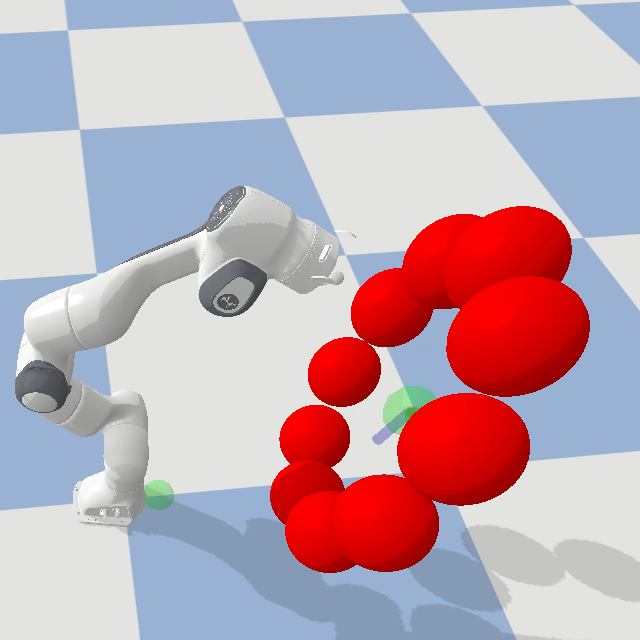
\includegraphics[width=0.8\textwidth]{task1_1.png}
        \caption{\reachinginring{}}
        \label{fig:reachinginring}
    \end{subfigure}
    \begin{subfigure}[b]{0.35\linewidth}
        \centering
        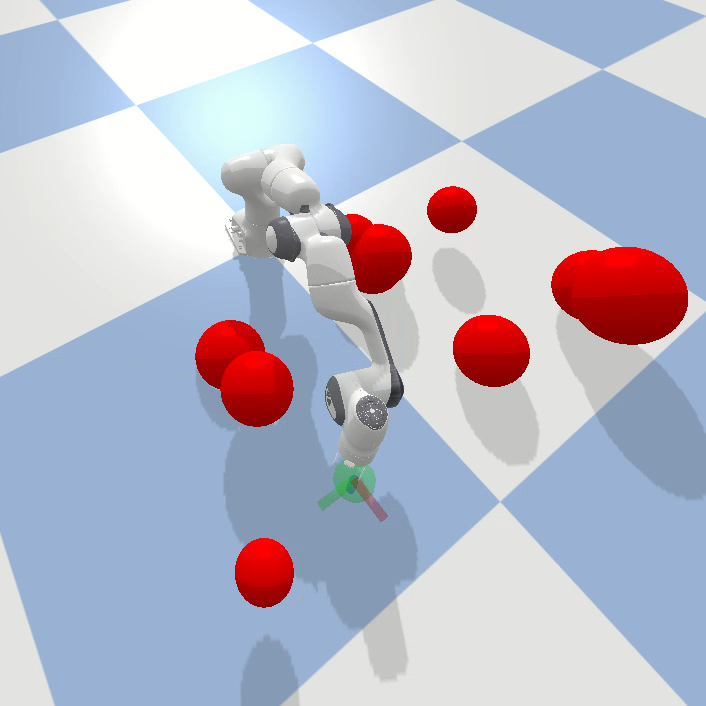
\includegraphics[width=0.8\textwidth]{task2_2.png}
        \caption{\reachingontable{}}
        \label{fig:reachingontable}
    \end{subfigure}
    \label{fig:tasks}
\end{figure}
%
\begin{figure}
    \centering
    \begin{subfigure}[b]{0.49\linewidth}
        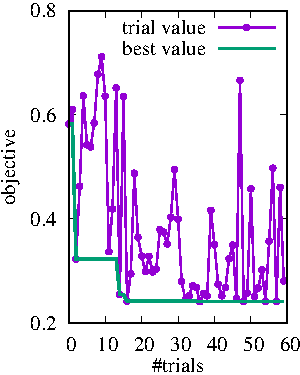
\includegraphics[width=1\textwidth]{history_panda_ring}
    \end{subfigure}
    \begin{subfigure}[b]{0.49\linewidth}
        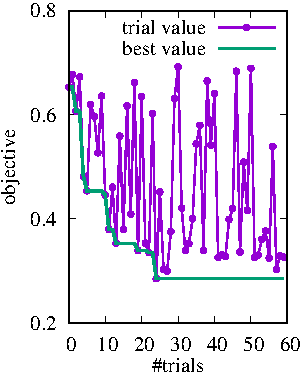
\includegraphics[width=1\textwidth]{history_panda_ring_real}
    \end{subfigure}
    \captionsetup{belowskip=-20pt}
    \caption{Optimization history for simulation (left) and real world (right) for panda robot in 
        \reachinginring{} scenario.}
    \label{fig:history}
\end{figure}

\subsection{Importance of tuning}
\label{sub:importance_tuning}
%
We compare the autotuned parameters with seven random parameter sets from the
search space and a manually tuned parameter set that we obtained through
expertise in previous works like \cite{Spahn2022}.
%
In this experiment, tuning and testing are performed on the test scenario
\reachinginring{}. Tuning is crucial for optimization
fabrics, as the performance with a random parameter set cannot compete with
tuning, \cref{fig:results_manual_random_autotune}. This result was expected and
should only demonstrate that the right parameter set is required to deploy this
method. Autotuned parameters reach a similar performance to the expert. This
result highlights the importance of tuning for optimization fabrics and shows
that autotuning is an effective way to obtain parameter sets for novice users
of optimization fabrics.
%
\begin{figure}
    \centering
    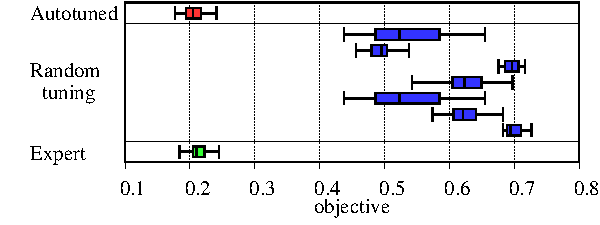
\includegraphics[width=\linewidth]{tuned_vs_random_plot}
    \caption{Evaluation for scenario \reachinginring{} autotuned parameters and compared
        to random parameter selection and manual tuning. Autotuning is able to 
        systematically outperform random parameter sets and reach expert level tuning.}
    \label{fig:results_manual_random_autotune}
\end{figure}

\begin{figure}
    \centering
    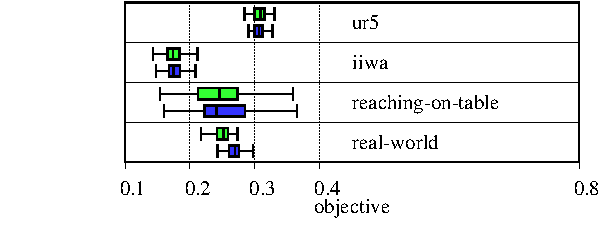
\includegraphics[width=\linewidth]{cross_validation_horizontal_plot}
    \captionsetup{belowskip=-20pt}
    \caption{
   %     Results for cross-evaluations. We evaluate the performance of
   %     the tuning with the panda robot on the \reachinginring{} case 
   %     in simulation, in the real world, and with two
   %     different robots and compare it to autotuning in the changing scenarios.
        The autotuned for the panda robot in simulation for the
        \reachinginring{} scenario on modified scenarios (blue) is compared to
        autotuned parameter sets obtained on these scenarios directly (green).
        Exchanging the robot (ur5, iiwa) and changing the scenario
        (\reachingontable{}) results in a very small loss in performance, while
        the loss is higher when parameters are transferred between simulation
        and real world (real-world).
    }
    \label{fig:cross_evaluation}
\end{figure}
%
%
\subsection{Cross validation: Transfer across robots}
\label{sub:cross_validation_robots}
%
Without any retuning, we deploy the symbolic optimization fabrics planner tuned
on the \panda{} on two other robots with similar specifications (Kuka LBR IIwa
7, Universal Robot UR5) and compare the performance with tuning performed on
the respective robot. 
Specifically, we do not change the leaf geometries and energies but change
differential maps according to relevant collision links on the robot at hand.
From \cref{fig:cross_evaluation}, we conclude that tuning is independent of the
robot. This can be explained by the fact, that optimization fabrics are a
purely geometric approach to trajectory generation and the different
dimension of the robots do not change the dynamical system enforced onto the
robot.
%
\subsection{Cross Validation: Transfer across scenarios}
\label{sub:cros_validation_tasks}
%
In the third experiment, we evaluate how well an autotuned parameter set
transfers to a different scenario. In the specific example, we use the tuning
obtained from the \reachinginring{} case and test it on \reachingontable{}.
Performance can be transferred smoothly if the objective remains the same, see
\cref{fig:cross_evaluation}. However, note that different scenario might
require generally slower motion because of a more crowded environment. Such a
step would require to retune the parameters according to the new objective.
%
\subsection{Cross Validation: Transfer real world}
\label{sub:cross_validation_transfer_real_world}
%
%
As optimization fabrics are a geometric method \cite{Wyk2022}, they should be
independent of the robot embodiment. Relying on the low-level controller. In
this paper, we investigate how the performance is affected by the transfer from
the simulation environment to the real world. 
Performance benefits from tuning in the real world highlight that low-level
controller differences affect the behavior, see \cref{fig:cross_evaluation}.
Specifically, the accumulated distance to the goal is increased ($0.14$m tuned
in the real world vs $0.16$m tuned in simulation) when tuning is transferred
between simulation and real world. Thus, there is added value in tuning in the
real world. Our framework offers to quickly tune fabrics in the real-world
using the \textit{fabrics-ros-bridge}. With relaxed performance requirements, it
is sufficient to tune in simulation.%

\subsection{Cross Validation: Transfer mobile manipulator}
%
%
Finally, we qualitatively test the performance of the tuning method on a real
mobile manipulator with 10 degrees of freedom. After only $N=30$ trials, the
robot was able to perform coupled mobile manipulation based on a visual
servoing approach \cite{chaumette2016visual}. Symbolic optimization fabrics are
especially suited for visual servoing as their symbolic character allows them
to constantly update the position of the goal. A video of this experiment is
attached to the paper.

\begin{figure}
    \centering
    \begin{subfigure}{0.5\linewidth}
        \centering
        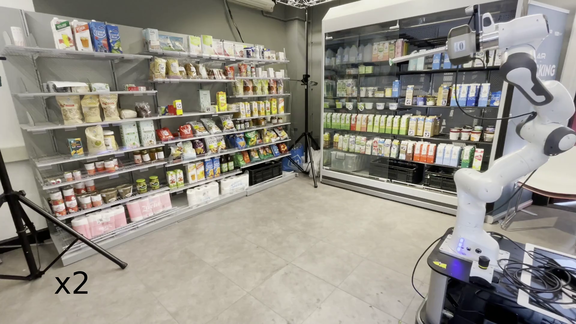
\includegraphics[width=.95\linewidth]{image_00002.png}
        \label{fig:my_label}
    \end{subfigure}%
    \begin{subfigure}{0.5\linewidth}
        \centering
        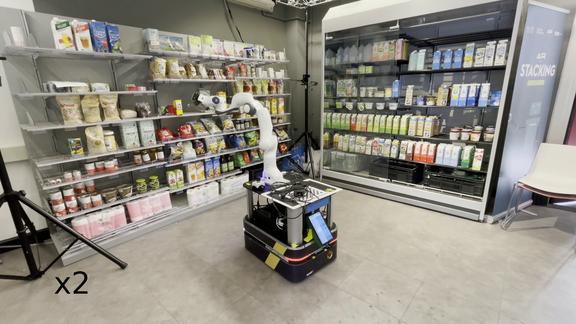
\includegraphics[width=.95\linewidth]{image_00005.png}
        \label{fig:my_label}
    \end{subfigure}
    \par\smallskip
    \begin{subfigure}{0.5\linewidth}
        \centering
        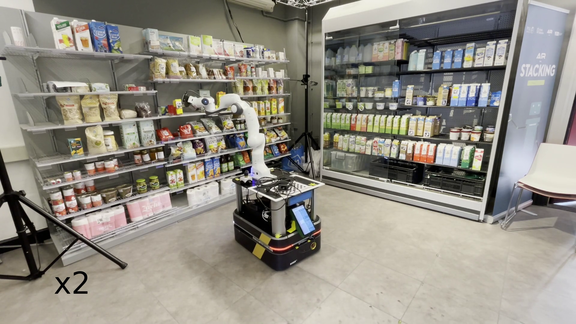
\includegraphics[width=.95\linewidth]{image_00006.png}
        \label{fig:my_label}
    \end{subfigure}%
    \begin{subfigure}{0.5\linewidth}
        \centering
        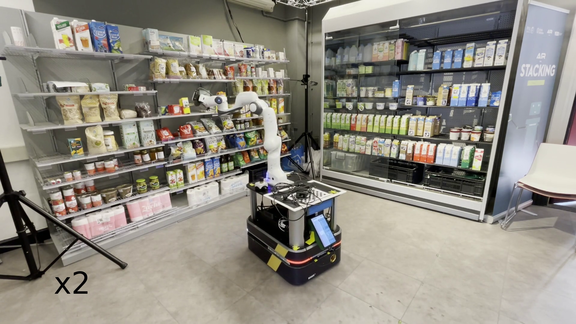
\includegraphics[width=.95\linewidth]{image_00007.png}
        \label{fig:my_label}
    \end{subfigure}%
    \captionsetup{belowskip=-10pt}
    \caption{Trajectory generation with optimization fabrics for mobile manipulator using visual serving for product picking.}
    \vspace{-10pt}
\end{figure}
%




\section{Conclusion}
\label{sec:conclusion}

This paper introduces several approaches to surpass explicit environment
representations, employing three distinct implicit representations within the
\ac{fabrics} framework. The study demonstrates that these techniques notably
reduce demands and constraints on perception pipelines, while maintaining a low
computational load on the planner. Consequently, the proposed methods enable the
application of analogous strategies in both dynamic and static environments.
The outcomes underline the successful integration of numerical gradients,
frequently accessible in trained models, into the symbolic implementation of
\ac{fabrics} detailed in \cite{Spahn2022}. Future endeavors should concentrate
on incorporating more implicit robot representations as outlined in
\cite{Liu2022regularized,Koptev2023neural} into this framework. While this work refrains from
delving into dynamic environmental dynamics, an exploration of the potential
synergies between the implicit representations introduced here and the findings
from \cite{Spahn2022} is a promising avenue for investigation.


\newpage
